\documentclass[acmtog]{acmart}
%acmtog if we're feeling a little funky ;)

\usepackage{booktabs, braket} % For formal tables
\usepackage{cleveref}

\settopmatter{printacmref=false} % Removes citation info after abstract
\renewcommand\footnotetextcopyrightpermission[1]{} % removes footnote with conference informat\textbf{}ion in first column
\usepackage{fancyhdr}

\DeclareMathOperator{\X}{\mathbb{X}}		     % expected value
\DeclareMathOperator{\tr}{\text{tr}}		     % expected value
 
\pagestyle{fancy}
\fancyhf{}
\lhead{Czekanski \& Witter, Fall 2019}
\rfoot{\thepage}

%\pagestyle{plain} % removes running heades

% Use the "authoryear" citation style, and make sure citations are in [square brackets].
\citestyle{acmauthoryear}
\setcitestyle{square}

% A useful command for controlling the number of authors per row.
% The default value of "authorsperrow" is 2.
\settopmatter{authorsperrow=1}

\begin{document}


% Title. 
% If your title is long, consider \title[short title]{full title} - "short title" will be used for running heads.
\title{Implementing a Semidefinite Program Solver to 
Find the Optimal Quantum Query Complexity
of Boolean Functions}

% please leave the subtitle!
\subtitle{Middlebury College, Fall 2019}

% Authors.
\author{Michael Czekanski}
\affiliation{%
  \institution{Middlebury College}}

\author{R. Teal Witter}
 \affiliation{%
   \institution{Middlebury College}}

\maketitle

% a couple of paragraphs describing your project
\section*{Abstract}

The development of quantum algorithms is an important area
of research as the creation of large quantum computers
becomes more feasible. Quantum computers can accomplish
certain tasks more efficiently than classical computers by
taking advantage of certain properties of quantum mechanics.
The runtime of a quantum algorithm on a given input is
thought to be well approximated by the quantum query
complexity of the algorithm on the input. We build on
existing research that represents optimal adversary bounds
on quantum query complexity for boolean functions as
semi-definite programming problem. Specifically, we aim to
create a tool that finds these optimal bounds for a given
boolean function via semi-definite programming more
efficiently than general solvers by taking advantage of the
structure in each of these problems.

We store our coding implementation and work at
\url{https://github.com/rtealw/Optimal-Quantum-Algorithms}.


% the other sections
\section{Introduction}

An important topic in quantum computing is
to determine the problems for which quantum
computers can outperform classical computers.
To avoid technical problems in the comparison of 
computers--the largest
of which is that large-scale quantum computers
currently do not exist--we turn to theoretical
analysis to characterize the efficiency of 
quantum and classical algorithms.

In this paper, we consider the query model of computation
to place an asymptotic lower bound on runtime.
The query complexity of a function 
is the number of times we must examine the
contents of the input string to determine the correct
output of the function. 
Each query of the given function takes a certain amount of time, therefore the query
complexity places a lower bound on runtime asymptotically. It's possible that the
implementation of the algorithm has a larger asymptotic runtime than query
complexity only if the post-processing of the query results takes more time than the
queries themselves.

To give a concrete example of query complexity,
recall the canonical OR function.
The $n$-bit OR
function returns $0$ if there are only $0$'s in the input
string and $1$ if there are any $1$'s in the input string.
A classical algorithm must check that
every single bit of the input is a $0$ to return $0$.
Therefore the classical query complexity of the $n$-bit OR
function is $n$. 
However, the quantum algorithm Grover's
search can solve the function OR in $\sqrt{n}$ queries
\cite{grover1996fast}. In the case of OR, we conclude that
the quantum algorithm outperforms the classical algorithm.

For an arbitrary function $f$,
Reichardt presents a semidefinite program (SDP)
whose solution corresponds to the optimal quantum query complexity
of $f$ \cite{reichardt2009span}.
In addition, the solution of the same SDP can
be used to construct a span program that, when run
on a quantum computer, meets the optimal quantum query complexity.

Our contribution is an SDP solver
that finds the optimal quantum query complexity
and query optimal quantum algorithm for given Boolean functions.
While the SDP can be solved for arbitrary functions,
we limit the scope of our work to Boolean functions.

While there are many SDP solver libraries such as CVXOPT and
SDPA for convex optimization problems,
none easily support solving Reichardt's SDP
\cite{cvxopt, SDPA}.
As a result, we develop an implementation that solves the SDP
and includes optimizations specific to our problem formulation.
We first convert Reichardt's form into the standard SDP form
as described by Boyd \cite{boyd2004convex}, which we verify here.
To solve the SDP, we implement Wen et al.'s alternating direction method (ADM)
algorithm in order to exploit the sparsity of our SDP
and then optimize the functions and data structures we use
to speed up our program \cite{adm}. 

Our program takes as input a set of bitstrings $D$
and a Boolean function $f: D \rightarrow \{0,1\}$. 
By solving Reichardt's SDP problem with
Wen et al.'s ADM algorithm,
we return the optimal quantum query complexity of $f$
and a quantum algorithm that meets this query complexity.
We hope that our solver proves useful
for researchers constructing optimal quantum algorithms.

\section{Methodology}\label{sec:method}

Consider the function $f: D \rightarrow E$ where $D
\subseteq {\{0,1\}}^n$ and $E \subset {0,1}$. We aim to find an
optimal bound on quantum query complexity using semidefinite
programming. From previous work,
we can formulate the problem as in \cref{eq:reichardtObj} where
$f_{\text{bound}}$ represents the optimal bound for the function
$f$ with the input size $n$ \cite{reichardt2009span}.
Let $F$ be the set of $(y,z)$ such that $f(y) \neq f(z)$.
Then the objective function of the SDP is
\begin{align} \label{eq:reichardtObj}
    f_{\text{bound}} = M(\X) = \max_{y \in D} \sum_{j \in [n]}
    \bra{y,j}\X\ket{y,j} 
\end{align}
subject to constraints
\begin{align}\label{Eq:semi1}
    \X \succcurlyeq 0 
\end{align}
and
\begin{align}\label{Eq:off-diag}
    \forall (y,z) \in F \sum_{j \in [n]: y_j \ne z_j} 
    \bra{y,j} \X \ket{z, j} = 1.
\end{align}
Our goal is to minimize $M$ by finding the optimal value of $\X$.

We construct the matrices in the SDP definition.
Observe that $\X$ is a $n2^n \times n2^n$ matrix 
because there are $2^n$ possible inputs each of length $n$. 
Think of $\X$ as containing chunks of size 
$n \times n$ where each chunk corresponds to an element of $D$. % x $D$.
Below we consider $\X$ of the OR function with one bit inputs,
\begin{align}
    \X = \left[
    \begin{matrix}
        1 & 1 \\
        1 & 1
    \end{matrix}
    \right]
    \nonumber
\end{align}
%\begin{align}
%   X = \left[ \begin{matrix}
%   \left[ \begin{matrix} (0,0)\end{matrix} \right] & \left[
%   \begin{matrix} (0,1)\end{matrix} \right] \\ \\
%   \left[ \begin{matrix} (1,0)\end{matrix} \right] & \left[
%   \begin{matrix} (1,1)\end{matrix} \right] \\
%    \end{matrix} \right]
%\end{align}

Our objective function \cref{eq:reichardtObj} is
the maximum trace of the diagonal sub-matrices. The
first constraint \cref{semi1} is that $\X$ is positive
semidefinite. The final constraint \cref{semi2} states that
diagonal entries where the input bits differ
of each sub-matrix where the Boolean outputs are not equal must sum to one.

Given this non-traditional formation of the semidefinite programming problem, we first convert the problem into an equivalent problem in standard form as defined by Boyd \cite{boyd2004convex}:
\begin{align}\label{Eq:boyd_obj}
    M(\X) = tr(C\X) 
\end{align}
subject to
\begin{align}
    \X \succcurlyeq 0   
\end{align}
and for $i \in \{1,...,|F|\}$
\begin{align}\label{Eq:trace}
    \tr(A_i \X) = b_i. 
\end{align}


To make these two problems equivalent we first note that
conditions \cref{Eq:semi1} and \cref{Eq:off-diag} are
the same.
To equate conditions \cref{Eq:off-diag}
and \cref{Eq:trace}, we define the set of matrices
$A_i$ and
scalars $b_i$ where $i \in [|F|]$.
We set $b_i$ equal to $1$ to satisfy \cref{Eq:off-diag}.
Observe that the sum in condition \cref{Eq:off-diag}
iterates through a portion of the matrix $\X$ diagonally.
Thus we can define a set of matrices where the matrix 
$A_i$ contains only 1s and 0s 
such that $A_i \X$ puts the off-diagonal values we want
to sum onto the diagonal.
Therefore the trace of this new matrix $A_i \X$ 
will be equal to the sum in \cref{Eq:off-diag}.

For example, consider a matrix $X$ where
\begin{align}
    X = \left[ \begin{matrix} 1 & 2 \\ 3 & 4 \end{matrix} \right] \nonumber
\end{align}
and suppose we want to put the top right value $2$ on the diagonal.
We could define $A$ as below:

\begin{align}
    A = \left[ \begin{matrix} 0 & 0 \\ 1 & 0 \end{matrix} \right] \nonumber
\end{align}

Therefore,
\begin{align}
    A \cdot X = \left[ \begin{matrix} 2 & 0 \\ 4 & 0 \end{matrix} \right] \nonumber
\end{align}
and subsequently,
\begin{align}
    \tr(A \cdot X) = 2. \nonumber
\end{align}

Through a similar construction we can build a set of matrices 
$A_i$ for each element of $F$ such that setting $b_i = 1$ 
creates an equivalent constraint to \cref{Eq:off-diag}.
Having now created $A_i$ and $b_i$ for $i = 1,2,...,
|F|$, we have defined constraints equivalent to eq.
\ref{Eq:semi1} and eq. \ref{Eq:off-diag} thus creating
a SDP constraints in Boyd's form that are equivalent to
Reichardt's form.

Our set of $A_i$ now satisfies \cref{Eq:off-diag}.
The problem is that \cref{Eq:boyd_obj}
does not have a maximum in the way \cref{eq:reichardtObj}
requires.
Our solution is to introduce slack variables
that enforce that our objective function is the maximum.
The big picture is that we construct a new
from our original $\X$,
\begin{align}
    \Xb =
    \left[
    \begin{matrix}
    \X & 0 \\
    0 & S
    \end{matrix}
    \right] \nonumber
\end{align}
%\begin{equation}
%    \Xb = \left[\begin{matrix} \X \cdots \cdots 0 \\
%                                \vdots \ddots \vdots \\
%                                0 \cdots \cdots z  \end{matrix}
%                                \right]  
%\end{equation}
where $S$ is a diagonal matrix
with objective function $z$ on the bottom right
and slack variables $s_i$ for $i \in [|D|]$
along the rest of the diagonal.

We guarantee that $z$ is the maximum
diagonal chunk of $\X$
by generating another set of matrices 
$\Ap_i$ and scalars $\bp_i$ for $i \in [|D|]$
where $\bp_i = 0$.
For each element of $D$, define a $c_i$ such that
\begin{align}
    c_i = \sum_{j \in [n]} \bra{y,j}\X\ket{y,j}
    \nonumber
\end{align} 
where $y$ is the $i^{th}$ element of $D$.
Our goal is to enforce that $z$ is the maximum $c_i$.
By requiring that $s_i + c_i = z$ and using
the fact that $s_i$ is positive
($\Xb$ is semidefinite so $S$ is as well),
we can keep $z$ larger than or equal to $c_i$.
The semidefinite program minimizes $z$
by our choice of $C$ so $z$ meets the maximum $c_i$.

To enforce $s_i + c_i = z$, define $\Ap_i$ as a diagonal
matrix  with 1s along the chunk
corresponding to the $i^{th}$ input,
1 in the entry corresponding to $s_i$,
and -1 in the entry corresponding to $z$.
In a slight abuse of notation, we show an example
of $\Xb A_i$.
\begin{align}
\left[\begin{matrix} c_i & 0 & 0 \\
                    0 & s_i & 0 \\
                    0 & 0 & z \end{matrix} \right]
\left[\begin{matrix} 1 & 0 & 0 \\
                    0 & 1 & 0 \\
                    0 & 0 & -1 \end{matrix} \right]
= \left[\begin{matrix} c_i & 0 & 0 \\
                    0 & s_i & 0 \\
                    0 & 0 & -z \end{matrix} \right]
            \nonumber
\end{align}
Notice that the trace of $\Xb A_i$
is $c_i + s_i - z$.
By setting $\bp_i = 0$, we have that $z$ is
greater than or equal to $c_i$.

The final matrix we define is $C$.
Our goal is to select out $z$ from $\Xb$
so $C$ has a single non-zero value in the 
entry corresponding to $z$.
\begin{align}
    C = \left[\begin{matrix} 0  \cdots 0 \\
                                \vdots \ddots \vdots \\
                                0 \cdots  1  \end{matrix}
                                \right]  
                                \nonumber
\end{align}

We will now prove that using our construction,
$z = \max\{c_1, c_2, ... c_{|D|}\}$ in the optimal $\Xb$

Notice that because our matrix $\Xb$ is semidefinite 
and diagonal, all of its diagonal entries are non-negative. 
Assume for contradiction that $z < c_i$
for some $i \in \{1,2,..., |D|\}$.
Therefore $z < c_i + s_i$ since $s_i \geq 0$.

By our constraint, $z = c_i + s_i$, 
meaning that $z < z$, a contradiction! 
Therefore it must be the case that $z$ is an 
upper bound of the traces of our sub-matrices $c_i$. 

Now assume for contradiction that $z \ne  \max\{c_1, c_2, ...
c_{|D|}\}$. We know that $z$ is an upper bound so we only need to
show that there is no upper bound of this finite set that is less
than $z$ to show it is the maximum. Our assumption is equivalent to
the statement that there does not exist a constant $a$ such that $a
> c_i \forall i$ and $a < z$. If $a$ did exist, then there would
exist an $\Xb$ that also satisfies all of our constraints,
but with $a$ in the bottom right most entry instead of $z$. This
would mean that our objective function was improved over our
initial matrix as $a < z$, meaning that the $\Xb$ we found
is not optimal: a contradiction. We conclude that our constraints
are equivalent to those outlined by Reichardt, while matching the
form of Boyd.

Once given a function $f$ and all possible inputs to the
function of length $n$ ($D$), we can then define matrices
$C, A_i, \Ap_i$ and vectors $b_i, \bp_i$ such that the solution of Boyd's SDP
produces the solution of the Reichardt's SDP which
produces the optimal bound of quantum query complexity for
arbitrary Boolean functions.
\section{Results}

\subsection{Step-by-step Example with OR}
Recall the two bit function OR which returns $1$ if there
is at least a single $1$ in the input and returns $0$ otherwise.
To understand Reichardt's formulation and the conversion
to Boyd's standard form, consider as inputs to our tool
the case with function $f: D \rightarrow E$ where
$D \subseteq {\{0,1\}}^2$ and $E =\{OR(x): x \in D \}$.
Let $F$ be the set of $(y,z)$ such that $f(y) \neq f(z)$. In this
case, $F = \{(00,01), (00,10), (00,11), (01,00), (10,00), (11,00)\}$

Let
\begin{align}
\X = \begin{blockarray}{ccccc}
\qquad & 00 & 01 & 10 & 11 \\
\begin{block}{c[cccc]}
  00 & X_{(00,00)} & X_{(00,01)} & X_{(00,10)} & X_{(00,11)}\\
  01 & X_{(01,00)} & X_{(01,01)} & X_{(01,10)} & X_{(01,11)}\\
  10 & X_{(10,00)} & X_{(10,01)} & X_{(10,10)} & X_{(10,11)}\\
  11 & X_{(11,00)} & X_{(11,01)} & X_{(11,10)} & X_{(11,11)}\\
\end{block}
\end{blockarray}. \nonumber 
\end{align}


The objective function of the SDP is
\begin{align} \label{eq:reichardtObj} 
    f_{\text{bound}} &= M(\X) = \max_{y \in D} \sum_{j \in [n]}
    \bra{y,j}\X\ket{y,j} \nonumber \\
    &= \max\{ \tr{X_{(00,00)}}, \tr{X_{(01,01)}}, \tr{X_{(10,10)}}, \tr{X_{(11,11)}} \} \nonumber
\end{align}
subject to constraints
\begin{align}
    \X \succcurlyeq 0  \nonumber 
\end{align}
and
\begin{align}\label{specific_constraint}
    \forall (y,z) \in F \sum_{j \in [n]: y_j \ne z_j} 
    \bra{y,j} \X \ket{z, j} = 1.
\end{align}
Observe that \cref{specific_constraint}
is equivalent to
\begin{align}
    \tr{X_{(00,01)}} &= \tr{X_{(00,10)}} = \tr{X_{(00,11)}} = 1 \nonumber \\
    \tr{X_{(01,00)}} &= \tr{X_{(10,00)}} = \tr{X_{(11,00)}} = 1. \nonumber
\end{align}

Our goal is to minimize $M$, 
and thus $f_{\text{bound}}$ by 
finding the optimal value of $\X$. 
By running our SDP solver, we obtain 
$\X$ with an objective function value of $\sqrt{2}$.
\begin{align}
    \X = \left[ \begin{array}{cc|cc|cc|cc}
    0.7 & 0 & 0 & 0 & 1 & 0 & 0.5 & 0\\
    0 & 0.7 & 0 & 1 & 0 & 0 & 0 & 0.5\\
    \hline
    0 & 0 & 0 & 0 & 0 & 0 & 0 & 0\\
    0 & 1 & 0 & \sqrt{2} & 0 & 0 & 0 & 0.7\\
    \hline
    1 & 0 & 0 & 0 & \sqrt{2} & 0 & 0.7 & 0\\
    0 & 0 & 0 & 0 & 0 & 0 & 0 & 0\\
    \hline
    0.5 & 0 & 0 & 0 & 0.7 & 0 & 0.6 & 0\\
    0 & 0.5 & 0 & 0.7 & 0 & 0 & 0 & 0.6\\
    \end{array}
\right] \nonumber
\end{align}
We use our solution to construct the input
vectors to the span program.
Consider $L$ such that $L^\dagger L = \X$.
Then construct $\bra{v_{x,i}}$
for all $x \in D$, $i \in [n]$.
With \cref{input_vectors},
\begin{align}
I &= \left[\begin{array}{cc}
    \bra{1}\bra{v_{00,1}} & \bra{1}\bra{v_{00,2}} \\
    \bra{1}\bra{v_{01,1}} & \bra{0}\bra{v_{01,2}} \\
    \bra{0}\bra{v_{10,1}} & \bra{1}\bra{v_{10,2}}\\
    \bra{0}\bra{v_{11,1}} & \bra{0}\bra{v_{11,2}}\\
\end{array} \right] \nonumber \\
&= \left[\begin{array}{c|c|c|c}
    0 \cdots 0 & \bra{v_{00,1}} & 0 \cdots 0 & \bra{v_{00,2}} \\
    0 \cdots 0 & \bra{v_{01,1}} & \bra{v_{01,2}} & 0 \cdots 0\\
    \bra{v_{10,1}} & 0 \cdots 0 & 0 \cdots 0 & \bra{v_{10,2}}\\
    \bra{v_{11,1}} & 0 \cdots 0 & \bra{v_{11,2}} & 0 \cdots 0\\
\end{array} \right] \nonumber
\end{align}
The columns of $I$ are the columns
used in the span program. 
If we remove rows of $I$ corresponding to elements 
$ x \in D$ such that $f(x) = 1$
and columns of $I$ that are the 
all zero vector, we obtain an equivalent span program where
\begin{align}
I &= \left[\begin{array}{cccc}
   0 & 1 & 0 & 1 \\
\end{array} \right] \nonumber
\end{align}
and $\tau = 1$.
In both definitions of $I$, the left two partitions
correspond to the first bit in the
input, and the right two partitions correspond 
to the second bit of the input. For each
input bit, the relevant block of $I$ 
is broken into left and right halves, corresponding
to whether the bit is $0$ (left) or $1$ (right). 
It is clear from this matrix that if either input bit is
$1$ the function will return true and otherwise
will return false.

\subsection{Accuracy with OR}

\begin{figure}[H]
\centering
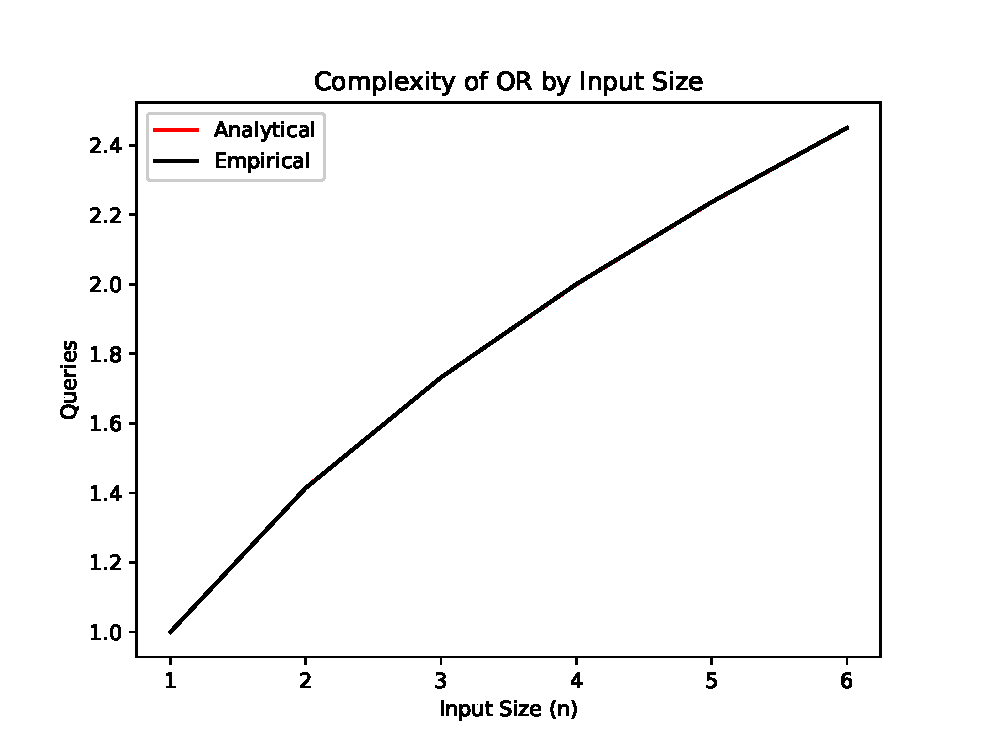
\includegraphics[scale=.5]{or_complexity}
\caption{The proven analytical optimal query complexity
and calculated empirical optimal query complexity by 
size of input bit string.}
\label{fig:or_complexity}
\end{figure}

We verify that our implementation works correctly
with results for OR on various input sizes.
The optimal quantum query complexity of OR
is $\sqrt{n}$ and, as demonstrated in
\cref{fig:or_complexity},
we the empirical results match the analytical
to the thousandth place.

\begin{figure}[H]
\centering
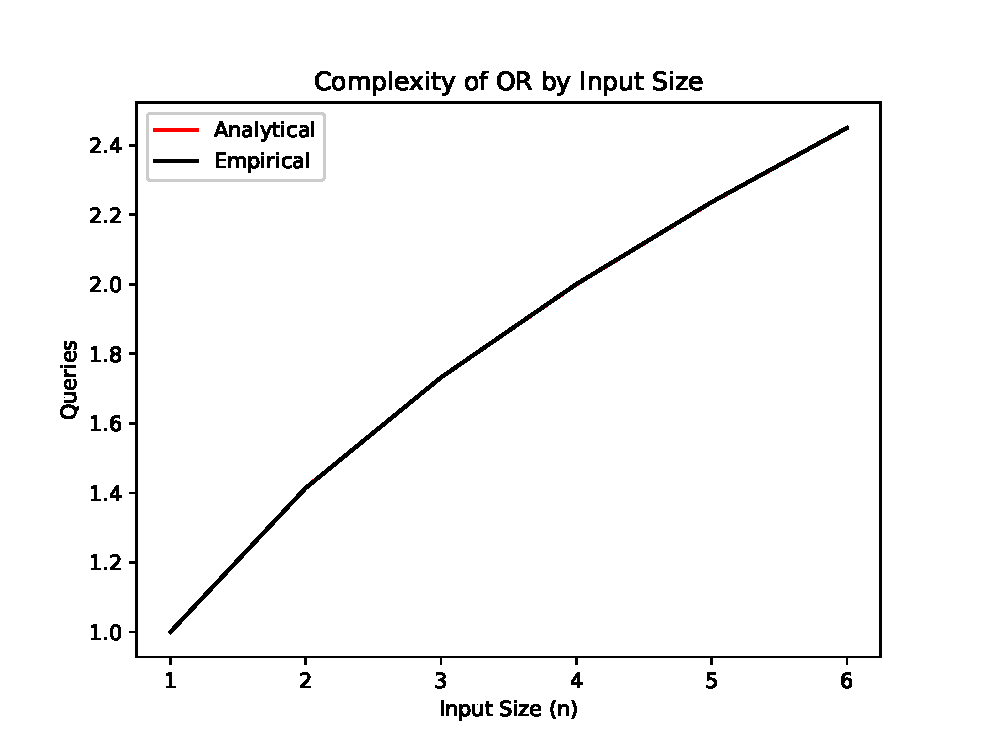
\includegraphics[scale=.5]{or_complexity}
\caption{The proven analytical optimal query complexity
and calculated empirical optimal query complexity by 
size of input bit string.}
\label{fig:or_complexity}
\end{figure}

\subsection{Runtime with OR}

\subsection{OR Function: Worst-case Boolean Inputs}\label{sec:speed}



\begin{figure}[H]
\centering
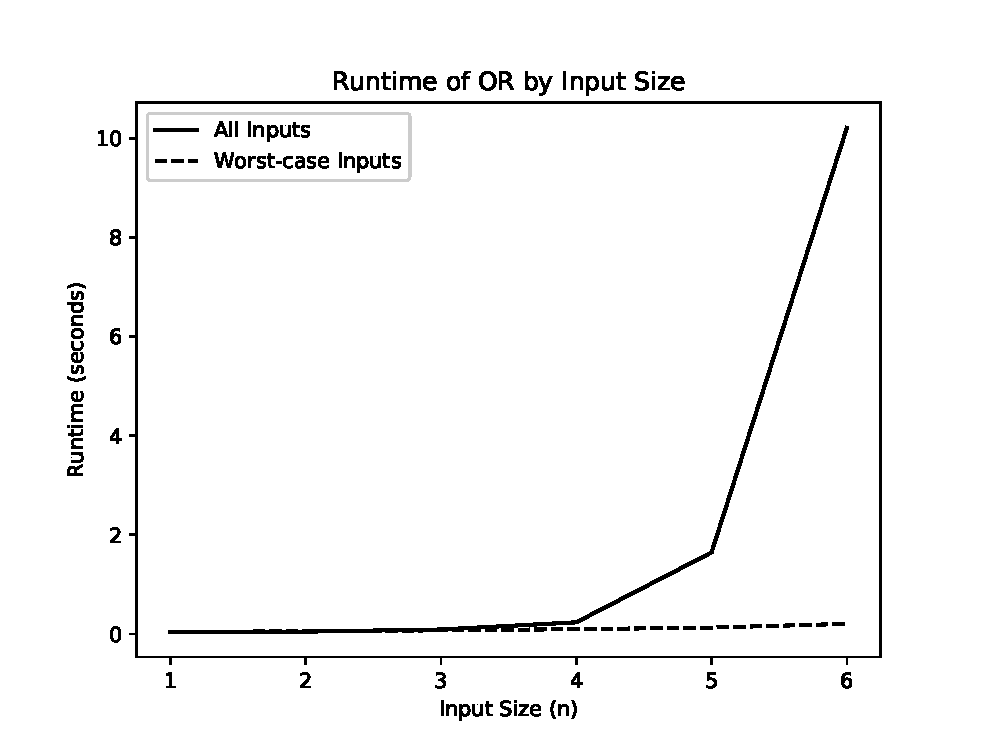
\includegraphics[scale=.5]{or_runtime}
\caption{Runtime of SDP solver by size of input strings.}
\label{fig:or_all_runtime}
\end{figure}

In \cref{fig:or_all_complexity}, observe that our algorithm
correctly calculates the optimal query complexity of the OR function (the
analytical and empirical lines are so close that one
is mostly obscured).
Our algorithm's performance is displayed in \cref{fig:or_all_runtime}.
We see that runtime grows exponentially with respect to input size as expected, 
given the exponential increase in the cardinality of the set $D$ of all
inputs of length $n$. 
We also see that our algorithm is accurately calculating the
optimal quantum query complexity of the OR function. 

The correctness of our algorithm is supported 
by it's performance on the OR function as it 
exactly matches the theoretical values. 
This is further supported by the proofs of Reichardt, 
Wen, and our Methodology section. 
In addition, we have made our source code 
available on GitHub for review. 
Given the correctness of our algorithm, 
we can address improvements to its runtime.

First, we can attempt to improve runtime while
maintaining the correctness of the algorithm. Later,
we might be able to alter the algorithm
mathematically to take advantage of the structure
given in SDP's formed from quantum algorithms. 
It has also been claimed that the dual of this semidefinite
programming problem yields the quantum algorithm with minimal query complexity.
However, this optimal solution to the dual may not be easily 
interpreted as an algorithm as there could be many optimal, feasible solutions. 
Semidefinite programming problems also don't guarantee the tightness of the dual,
as is the case in linear programming. 
These problems all pose potential areas of future expansion.

\subsection{OR Function: All Boolean Inputs}

A simple approach to speeding up the runtime of our
algorithm is to simply decrease the number of input
strings considered for a given input size $n$. It's
important that we still obtain a good approximation
of the correct answer, so we need to ensure that the
inputs we do analyze will lead to the correct result.
Because the bounds of our algorithm are adversarial,
meaning that they are worst-case bounds, we can opt
to only use the worst-case inputs.

Again returning to our OR example, the hardest inputs are
either entirely zeros, or contain only a single 1. 
Using these inputs, we can then run our algorithm to 
compare both runtime and precision of results.

The runtime is drastically improved over the all-case scenario. 
This result is not only shown via \todo{put both runtimes on the same figure and reference it here} of the graphs, 
but also in the x-axis because the speed up was so 
significant that we were able to solve for many more 
input sizes than in the all-case scenario. 
Looking at the optimal query complexities returned, 
we observe that we are still obtaining good 
approximations of the true value. 
We believe that more iterations could drastically 
improve the performance of the algorithm as well as 
improved stopping conditions. Instead of simply stopping 
after some number of iterations (in this case 100), 
we could look to see if the improvements to the objective 
function are negligible and conclude that the algorithm has converged.

\section{Conclusion}


\begin{acks}
The authors would like to thank Professors Shelby Kimmel
and Philip Caplan for their invaluable help and support. 
\end{acks}

% select the reference format (leave this)
\bibliographystyle{ACM-Reference-Format}

% specify the bibliography (.bib) file
% place your references in this bib file
\bibliography{main}

\end{document}